\documentclass[12pt]{article}
\usepackage{graphicx}
\usepackage{epstopdf}
\usepackage{booktabs}
\usepackage[table]{xcolor}
\usepackage{float}
\usepackage{caption}
\usepackage{hyperref}
\usepackage{adjustbox}
\usepackage{amsmath}
\usepackage{listings}
\usepackage[document]{ragged2e}
\usepackage{titling}
\usepackage{lipsum}

\author{Assignment 1 (Camera Calibration) \\ Vaishali Pal \\ 201407665}
\title{Computer Vision Assignment Report}
\date{\today}


\preauthor{\begin{flushright}\large} % makes author flush right
\postauthor{\end{flushright}}

\begin{document}
  \maketitle
  
\section{Introduction}
The purpose of this assignment is to be familiar with camera calibration. The algortithms used for this purpose are DLT, RANSAC, and Zhang's method.

\section{DLT}
DLT uses at least 6 image points to estimate the camera parameters. The points should not lie on a plane, else DLT will produce degenerate results.

\subsection{Code} 
\begin{lstlisting}[language=matlab]
    imagePoints = [ 488, 140, 1;
        404, 134, 1;
        388, 238, 1;
        493, 57, 1;
        407, 51, 1;
        474, 246, 1];

    worldPoints = [0, 36, 0, 1;
        36, 36, 0, 1;
        36, 0, 36, 1;
        0, 72, 0, 1;
        36, 72, 0, 1;
        0, 0, 36, 1];


    A = zeros(12, 12);
    k = 1;
    for i = 1:6
        imgPt = imagePoints(i, 1);
        A(k, 1:4) = -worldPoints(i,:);
        A(k,5:8) = zeros(1,4);
        A(k,9:12) = [imgPt*worldPoints(i,1),
         			imgPt*worldPoints(i,2),
         			imgPt*worldPoints(i,3), 
         			imgPt];
        k = k + 1;

        imgPt = imagePoints(i, 2);
        A(k,1:4) = zeros(1,4);
        A(k, 5:8) = -worldPoints(i,:);
        A(k,9:12) = [imgPt*worldPoints(i,1),
        			 imgPt*worldPoints(i,2),
        			 imgPt*worldPoints(i,3),
        			 imgPt];
        k = k + 1;
    end

    [U, S, V] = svd(A);
    singV = diag(S);
    [~, indx] = sort(singV);
    p = V(:, indx(1));
    p = reshape(p, [4,3])';
    estimatedImg = p*worldPoints';
    imgEst = round(estimatedImg ./ repmat(estimatedImg(3,:),3,1))';
    imagePoints
    H = p(:,1:3);
    invH = inv(H);
    [invR, invK] = qr(invH);
    R = invR';
    K = inv(invK);

\end{lstlisting}

\subsection{Input}
The input to DLT are image points and their correspondinf world coordinates. For this experiment, 6 image points have been chosen.

\subsection{Output}
There were no re-projection error for the chosen image coordinates. It has been observed that DLT gives very high accuracy in estimating the camera parameters and thus very low re-projection error. 

The image coordinates of the corner points were as follows:
\begin{lstlisting}[language=matlab]
 imagePoints = [ 488, 140, 1;
    404, 134, 1;
    388, 238, 1;
    493, 57, 1;
    407, 51, 1;
    474, 246, 1];
\end{lstlisting}
The projected image coordinates estimated from the camera matrix are as follows:
\begin{lstlisting}[language=matlab]
  487.9798  140.2380    1.0000
  404.0205  133.7647    1.0000
  387.9901  238.1065    1.0000
  493.0110   56.8638    1.0000
  406.9888   51.1346    1.0000
  474.0100  245.8923    1.0000
\end{lstlisting}

The parameters of the camera matrix are as follows:
\subsection{Camera Projection Matrix} 
\begin{lstlisting}[language=matlab]
P = [-0.0041   -0.0003   -0.0017    0.9102
     -0.0003   -0.0043    0.0007    0.4140
      0.0000   -0.0000   -0.0000    0.0019]
\end{lstlisting}
\subsection{Intrinsic Parameters}
\begin{lstlisting}[language=matlab]
K = [ 0.0007    0.0043   -0.0365
           0    0.0002   -0.0080
           0         0   -0.0002]
\end{lstlisting}
\subsection{Extrinsic Parameters}
\begin{lstlisting}[language=matlab]
R = [ -0.9070    0.1404   -0.3970
      -0.3594   -0.7495    0.5559
      -0.2195    0.6469    0.7303]
      
C = [ 54.9197
     -207.6365
     -632.9154]
\end{lstlisting}

\subsection{WireFrame of Estimated Points}
\begin{figure}[htp]
\centering
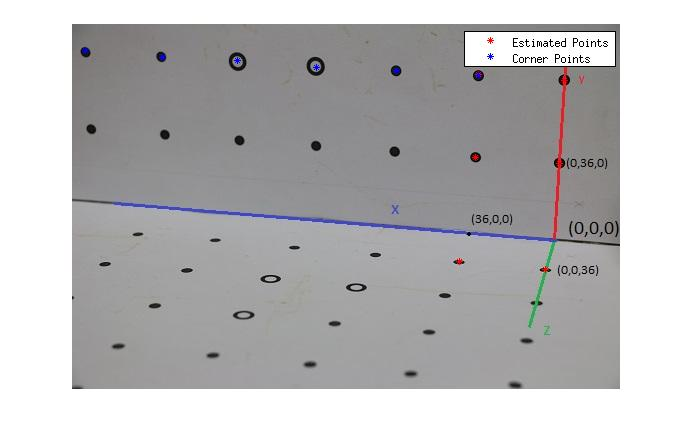
\includegraphics[width=1\textwidth]{wireFrameDLT2.jpg}\hfill
\end{figure}
 
\section{RANSAC}
Random sample consensus (RANSAC) is an iterative method to estimate parameters of a mathematical model from a set of observed data which contains outliers. RANSAC is used for camera calibration to estimate the camera matrix with the least re-projection error.
The best estimation of the camera matrix is chosen to be the one with minimum number of outliers.

The average reprojection error of the experiment by RANSAC is 11.7119.

\subsection{Code} 
\begin{lstlisting}[language=matlab]
imgPts = [14, 27, 1;
91, 34, 1;
166, 37, 1;
245, 44, 1;
325, 47, 1;
407, 52, 1;
493, 57, 1;
20, 104, 1;
94, 110, 1;
168, 117, 1;
245, 122, 1;
323, 128, 1;
404, 134, 1;
488, 140, 1;
398, 209, 1;
474, 246, 1;
465, 279, 1;
455, 316, 1;
444, 360, 1;
387, 236, 1;
304, 231, 1;
224, 223, 1;
114, 216, 1;
66, 210, 1;
34, 240, 1;
117, 246, 1;
200, 254, 1];  

worldPts = [216, 72, 0, 1;
180, 72, 0, 1;
144, 72, 0, 1;
108, 72, 0, 1;
72, 72, 0, 1;
36, 72, 0, 1;
0, 72, 0, 1;
216, 36, 0, 1;
180, 36, 0, 1;
144, 36, 0, 1;
108, 36, 0, 1;
72, 36, 0, 1;
36, 36, 0, 1;
0, 36, 0, 1;
36, 0, 0, 1
0, 0, 36, 1;
0, 0, 72, 1;
0, 0, 108, 1;
0, 0, 144, 1;
36, 0, 36, 1;
72, 0, 36, 1;
108, 0, 36, 1;
144, 0, 36, 1;
216, 0, 36, 1;
216, 0, 72, 1;
144, 0, 72, 1;
108, 0, 72, 1];

err = 0;
mnErr = 5000000;
p = zeros(3,4);
est = zeros(size(imgPts));

for iter = 1:1000
   indices = randperm(size(worldPts, 1), 6)
   P = DLT(imgPts(indices,:), worldPts(indices, :));
   estimatedImg = P*worldPts';
   imgEstimated = round(estimatedImg ./ repmat(estimatedImg(3,:),3,1));
   imgEstimated = imgEstimated';
   err = sum(sqrt(sum((imgPts - imgEstimated).^2,2)))/size(imgPts,1);
   if mnErr >= err
       p = P;
       mnErr = err;
   end
end

estimatedImg = p*worldPts';
imgEstimated = round(estimatedImg ./ repmat(estimatedImg(3,:),3,1));
imgEstimated = imgEstimated';
\end{lstlisting}

\subsection{Input}
The input to RANSAC are a set of 27 image and their correspoding world points. 
The actual image points are as follows:
\begin{lstlisting}[language=matlab]
    14    27     1
    91    34     1
   166    37     1
   245    44     1
   325    47     1
   407    52     1
   493    57     1
    20   104     1
    94   110     1
   168   117     1
   245   122     1
   323   128     1
   404   134     1
   488   140     1
   398   209     1
   474   246     1
   465   279     1
   455   316     1
   444   360     1
   387   236     1
   304   231     1
   224   223     1
   114   216     1
    66   210     1
    34   240     1
   117   246     1
   200   254     1
   \end{lstlisting}


\subsection{Output}

There are few errors in the estimation of image points from the camera matrix. This is due to radial distortion. 

The estimated image points are as follows
\begin{lstlisting}[language=matlab]
     3    24     1
    81    29     1
   160    35     1
   240    40     1
   323    46     1
   407    51     1
   493    57     1
     9   103     1
    85   109     1
   162   115     1
   241   121     1
   322   127     1
   404   134     1
   488   140     1
   401   213     1
   474   246     1
   464   275     1
   453   307     1
   440   343     1
   388   238     1
   304   230     1
   221   223     1
   141   216     1
   -16   202     1
   -50   226     1
   114   242     1
   199   250     1
   \end{lstlisting}
The parameters of the camera matrix are as follows:
\subsubsection{Camera Projection Matrix} 
\begin{lstlisting}[language=matlab]
P = [-0.0041   -0.0003   -0.0017    0.9102
     -0.0003   -0.0043    0.0007    0.4140
      0.0000   -0.0000   -0.0000    0.0019]
\end{lstlisting}
\subsubsection{Intrinsic Parameters}
\begin{lstlisting}[language=matlab]
K = [ 0.0043    0.0001   -0.0009
           0    0.0043   -0.0011
           0         0   -0.0000]
\end{lstlisting}
\subsubsection{Extrinsic Parameters}
\begin{lstlisting}[language=matlab]
R = [  -0.9754    0.0205   -0.2193
       -0.1107   -0.9062    0.4081
       -0.1904    0.4223    0.8862]
      
C = [ 54.9197
     -207.6365
     -632.9154]
\end{lstlisting}

\subsection{Output Image}
\begin{figure}[htp]
\centering
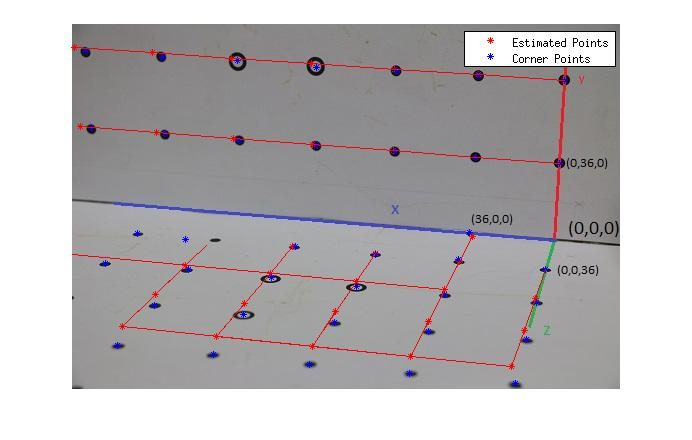
\includegraphics[width=1\textwidth]{wireFrameRANSAC.jpg}\hfill
\end{figure}
\clearpage


\section{Radial Distortion}

\subsection{Code for Distortion Parameter Estimation}
\begin{lstlisting}
imgPts = [14, 27, 1;
91, 34, 1;
166, 37, 1;
245, 44, 1;
325, 47, 1;
407, 52, 1;
493, 57, 1;
20, 104, 1;
94, 110, 1;
168, 117, 1;
245, 122, 1;
323, 128, 1;
404, 134, 1;
488, 140, 1;
398, 209, 1;
474, 246, 1;
465, 279, 1;
455, 316, 1;
444, 360, 1;
387, 236, 1;
304, 231, 1;
224, 223, 1;
114, 216, 1;
66, 210, 1;
34, 240, 1;
117, 246, 1;
200, 254, 1];  

I = imread('IMG_5464.JPG');
gray = rgb2gray(I);
rows = size(I,1);
cols = size(I,2);
d = min(rows, cols) / 2;
centerX = cols/2;
centerY = rows/2;
;
        
mnErr = 5000000;
estK1 = 0;
estK2 = 0;
estPts = [];
for k1 = -0.15:0.0001:0.1
    for k2 = -0.15:0.0001:0.1
        UnXList = [];
        UnYList = [];
        for i = 1:size(imgPts,1)
            xd = imgPts(i,1);
            yd = imgPts(i,2);
            %xd = (x - centerX);
            %yd = (y - centerY);
            r = sqrt((xd-centerX)^2 + (yd-centerY)^2);
            Lr = 1 + k1*r^1 + k2*r^2;
            xUn = xd/Lr;
            yUn = yd/Lr;
            UnXList = [UnXList;xUn];
            UnYList = [UnYList;yUn];
        end
        err = 0;
        for p = 1:size(UnXList,1)
            for q = p+1:size(UnXList,1)
                err = err + sqrt((UnXList(p) -
                 UnXList(q))^2 + (UnYList(p) -
                 UnYList(q))^2);
            end
        end
        if err < mnErr
            mnErr = err;
            estK1 = k1;
            estK2 = k2;
            estX = UnXList;
            estY = UnYList;
        end
    end
end
estK1
estK2
newPts = [estX, estY];
\end{lstlisting}


\subsection{Output}
The radial distortion parameter K1 and K2 are 0.1 and 0.1.
\subsection{Code for Radial Distortion Correction}
\begin{lstlisting}
function correctRadial2()%I, k, varargin)
I = imread('distort.jpg');
k = 0.1;


     for i=1:3
       I2(:,:,i) = imdistcorrect(I(:,:,i),k, [0,0]);
     end   
end

    function I3 = imdistcorrect(I,k, center)
    % Determine the size of the image to be distorted
    [M N]=size(I);
    %If Center is (0,0) then we use the center of the image, otherwise it
    %should will be the coordintes of the image center
    center = [round(N/2) round(M/2)];

    %center = [1592,656];
    % Creates N x M (#pixels) x-y points
    [xi,yi] = meshgrid(1:N,1:M);
    % Creates converst the mesh into a colum vector of coordiantes relative to
    % the center
    xt = xi(:) - center(1);
    yt = yi(:) - center(2);
    % Converts the x-y coordinates to polar coordinates
    [theta,r] = cart2pol(xt,yt);
    % Calculate the maximum vector (image center to image corner) to be used
    % for normalization
    R = sqrt(center(1)^2 + center(2)^2);
    % Normalize the polar coordinate r to range between 0 and 1 
    r = r/R;
    % Aply the r-based transformation
    
    s = r.*(1./(1+k.*(r.^2)));
    % un-normalize s
    s2 = s * R;
      
    % Convert back to cartesian coordinates
    [ut,vt] = pol2cart(theta,s2);
  
    u = reshape(ut,[M N]) + center(1);
    v = reshape(vt,[M N]) + center(2);
    tmap_B = cat(3,u,v);
    resamp = makeresampler('cubic', 'fill');
    I3 = tformarray(I,[],resamp,[2 1],[1 2],[],tmap_B,255);
    end

\end{lstlisting}

\subsection{Input Image}
\begin{figure}[htp]
\centering
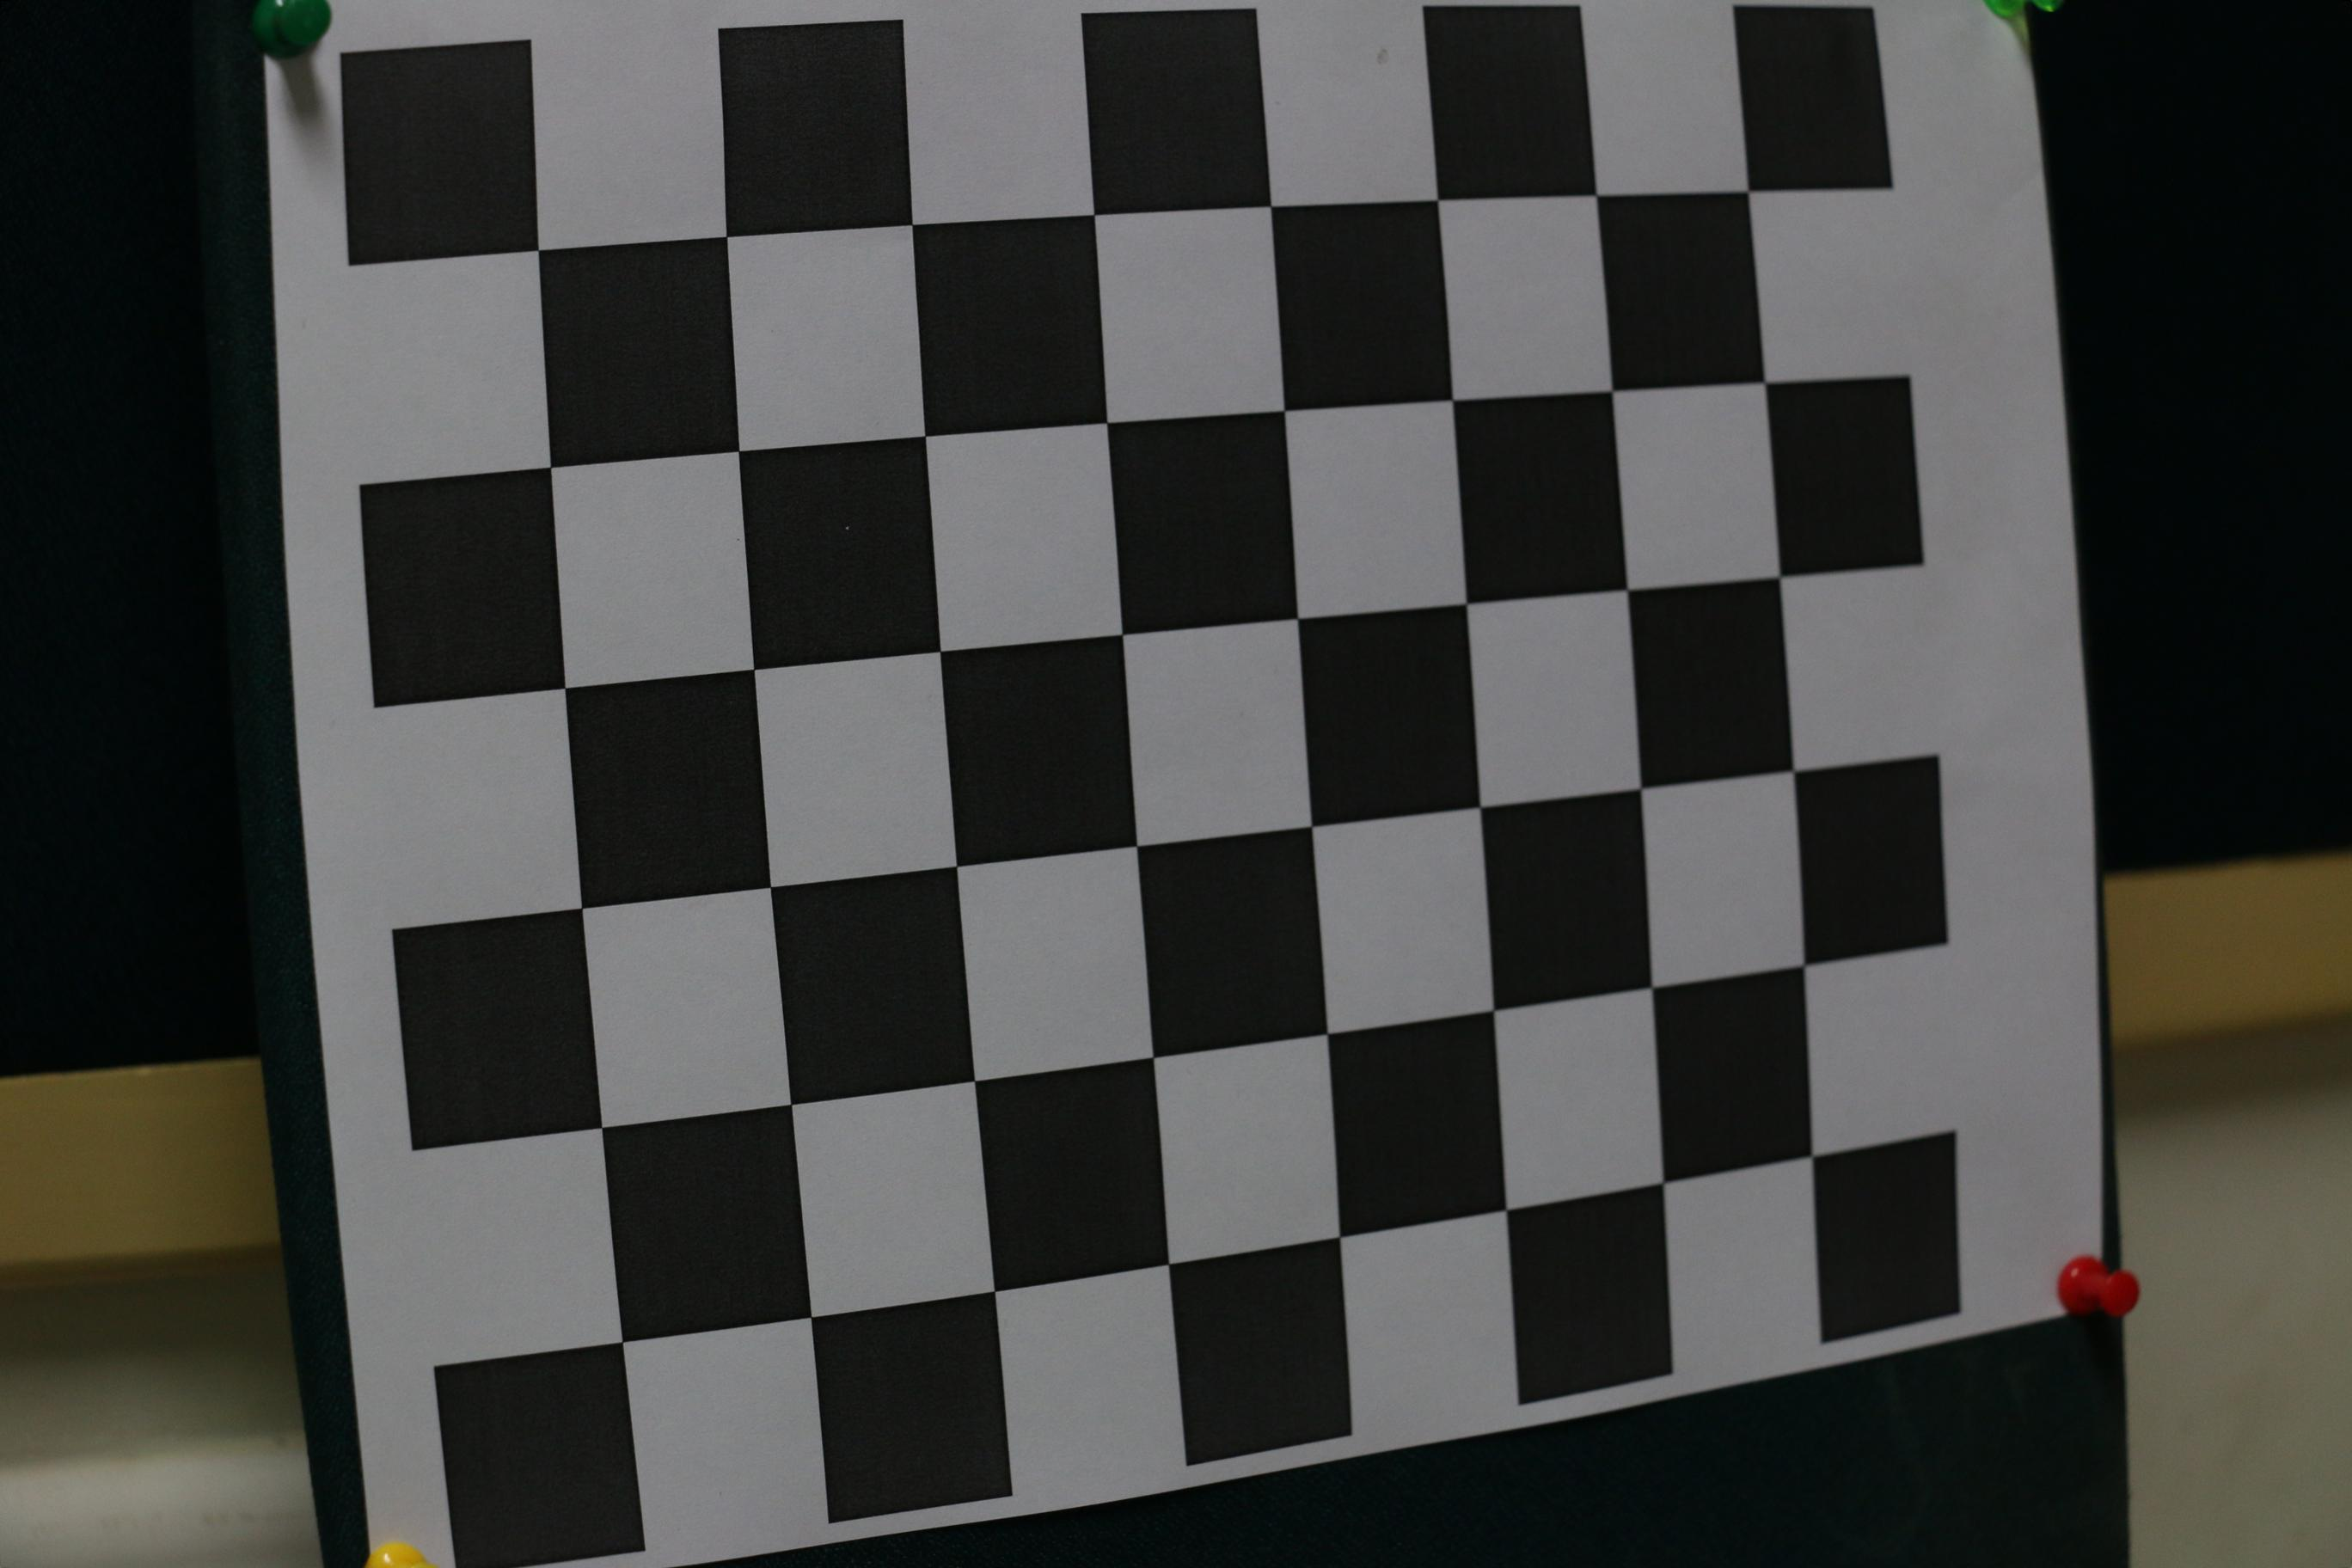
\includegraphics[width=1\textwidth]{distort.jpg}\hfill
\end{figure}
\clearpage
\subsection{Output Image}
\begin{figure}[htp]
\centering
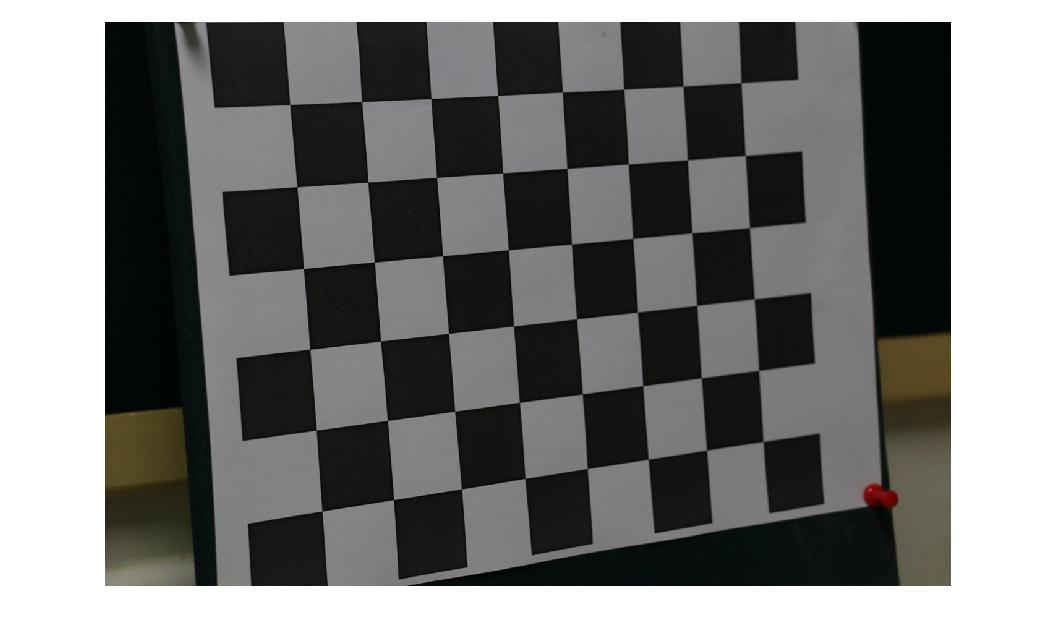
\includegraphics[width=1\textwidth]{undistored.jpg}\hfill
\end{figure}
\clearpage

\subsection{DLT after radial Distortion}
\subsubsection{Camera Projection Matrix}
\begin{lstlisting}
p =

   -0.0036   -0.0001   -0.0016    0.9110
    0.0001   -0.0046    0.0009    0.4123
    0.0000   -0.0000   -0.0000    0.0019

\end{lstlisting}

\subsection{Intrinsic Parameter}
\begin{lstlisting}
K =

    0.0036    0.0000    0.0014
         0    0.0046   -0.0009
         0         0   -0.0000
         
\end{lstlisting}
\subsection{Extrinsic Parameter}
\begin{lstlisting}
R =

   -0.7061   -0.1452   -0.6930
   -0.1138   -0.9428    0.3135
   -0.6989    0.3002    0.6492



C =

   32.4343
 -208.8298
 -637.8236
 \end{lstlisting}

\subsection{Radial Corrected Input Points}
\begin{lstlisting}
imagePoints = [ 499, 134, 1;
    407, 132, 1;
    389, 239, 1;
    508, 46, 1;
    414, 44, 1;
    482, 251, 1];
\end{lstlisting}

\subsection{Estimated Points}
 \begin{lstlisting}
imgEst =

  498.8616  135.4504    1.0000
  407.1516  130.6297    1.0000
  388.9188  239.6291    1.0000
  508.0671   45.1816    1.0000
  413.9260   44.7729    1.0000
  482.0855  250.3377    1.0000
\end{lstlisting}

The reprojection error is about 6.1488.

\subsection{Ransac after radial Distortion}
\subsubsection{Camera Projection Matrix}
\begin{lstlisting}
p =

   -0.0036   -0.0001   -0.0016    0.8110
    0.0001   -0.0046    0.0009    0.5723
    0.0000   -0.0000   -0.0000    0.0119

\end{lstlisting}

\subsection{Intrinsic Parameter}
\begin{lstlisting}
K =

    0.0036    0.0000    0.0014
         0    0.0046   -0.0009
         0         0   -0.0000
         
\end{lstlisting}
\subsection{Extrinsic Parameter}
\begin{lstlisting}
R =

   -0.8161   -0.1452   -0.6890
   -0.2038   -0.9428    0.6735
   -0.5900    0.5002    0.6492



C =

   30.8653
 -100.8298
 -700.8236
 \end{lstlisting}


\section{Camera Calibration using Zhang's Method}
Zhang's method finds the camera calibration from a number of images(at least 6) instead of a single image. For the experiment, 15 images were provided of which 8 were used by the algorithm. OpenCv has been used to estimate the camera matrix.

\subsection{Input}
The input to Zhang's method is a list of 15 checkerboard images at various distances and angles to the camera.

\subsection{Output}
The average re-projection error is 0.4764.

\subsection{Per View Re-projection Errors}
\begin{tabular}{|c|c|c|c|c|c|c|c|c|}
\hline
Views & 1 & 2 & 3 & 4\\
Error & 4.45612878e-01 & 4.16758776e-01 & 5.33244491e-01 & 5.22755444e-01 \\
\hline
Views & 5 & 6 & 7 & 8 \\
Error & 4.24562335e-01 & 3.42109889e-01 & 6.22883558e-01 & 4.48383838e-01 \\
\hline
\end{tabular}

\subsubsection{Distortion Coefficients}
\begin{tabular}{|c|c|c|c|c|}
\hline
3.5641444594248478e-01 & -7.6895267684771689e+00 & 0. & 0. &
    1.6732388239861839e+02 \\
    \hline
\end{tabular}
\subsubsection{Intrinsic Parameters}

\begin{lstlisting}
       
K = [2446.5393184376              0     499.5 
                   0 2446.539318437     332.5 
                   0          0            1]
\end{lstlisting}

\subsection{Extrinsic Parameters}
The rotation Matrix for the 15 views are as follows:
\\
R1
\begin{tabular}{|c|c|c|}
\hline
0.00328069473509518	& 0.998912619274484 &	0.0465060866580260 \\
0.999946317117785	& -0.00281989551069484 &	-0.00997051011166577 \\
-0.00982852606615983 &	0.0465363002772832 &	-0.998868245982357 \\
\hline
\end{tabular}

R2
\begin{tabular}{|c|c|c|}
\hline
-0.0356069985049111	& 0.973419778601566 &	-0.226243400533034 \\
0.999364049672338 &	0.0342504197102492 &	-0.00991992803279924 \\
-0.00190732272450052 &	-0.226452739830966 &	-0.974020286617827 \\
\hline
\end{tabular}

R3
\begin{tabular}{|c|c|c|}
\hline
0.0365368307623132	& 0.915017641760799 &	0.401755865251961 \\
0.999331230505276 &	-0.0328640307010605 &	-0.0160326923157348 \\
-0.00146687922384853 &	0.402072966950758 &	-0.915606453402747 \\
\hline
\end{tabular}

R4
\begin{tabular}{|c|c|c|}
\hline
0.0679651778772694 & 0.813136553118128 &	0.578091411957730 \\
0.996931132559000 &	-0.0779121015186385 &	-0.00761717608949197 \\
0.0388465124656002	& 0.576835028773496 &	-0.815936454663683 \\
\hline
\end{tabular}

R5
\begin{tabular}{|c|c|c|}
\hline
-0.0635202298042231 & 0.950205224343886 &	-0.305082303707057 \\
0.997860910669137 &	0.0652055572269334 &	-0.00467314297730612 \\
0.0154526167421529 &	-0.304726544521989 &	-0.952314522465928 \\
\hline
\end{tabular}

R6
\begin{tabular}{|c|c|c|}
\hline
0.0518669790804445 & 0.975973546685526 &	0.211625737213468 \\
0.947606152533138 &	0.0187868466181493 &	-0.318888121565368 \\
-0.315202151265520 & 0.217077614148076 &	-0.923864120568262 \\
\hline
\end{tabular}

R7
\begin{tabular}{|c|c|c|}
\hline
0.0401908020897435 &	0.927820004757500 &	0.370856762374877 \\
0.981616004448491 &	0.0326454995041404 &	-0.188053958141553 \\
-0.186587028589778 &	0.371596972718990 &	-0.909450917107746 \\
\hline
\end{tabular}

R8
\begin{tabular}{|c|c|c|}
\hline
-0.0623138318300953 &	0.949210800564852 &	0.308408564170458 \\
0.970019193571399 &	-0.0151294334591594 &	0.242556930113938 \\
0.234903704665855 &	0.314276878459485 &	-0.919809922320921 \\
\hline
\end{tabular}

R9
\begin{tabular}{|c|c|c|}
\hline
-0.0581970012124798	& 0.995199173414642 &	-0.0786874468049923 \\
0.949501926040635 &	0.0795228708827704 &	0.303516400630487 \\
0.308316722697616 &	-0.0570501379610603 &	-0.949571524564435 \\
\hline
\end{tabular}

R10
\begin{tabular}{|c|c|c|}
\hline
-0.0381270991079316 &	0.846413218016220 &	0.531160040553730 \\
0.939201173670841 &	-0.151165707588780 &	0.308301936783565 \\
0.341244017806800 &	0.510620791994029 &	-0.789188777856390 \\
\hline
\end{tabular}

R11
\begin{tabular}{|c|c|c|}
\hline
0.0107466817345443 &	0.918473568369743 &	0.395336329013470 \\
0.973493614925899 &	-0.0999396126037029 &	0.205723735944899 \\
0.228461573421442 &	0.382646544527417 &	-0.895202173495478 \\
\hline
\end{tabular}

R12
\begin{tabular}{|c|c|c|}
\hline
0.0119983079303003 &	0.956752028421313 &	0.290657180744796 \\
0.993540108380768 &	0.0213971684467383 &	-0.111446014828677 \\
-0.112845441403459	& 0.290116730462353 &	-0.950314784195370 \\
\hline
\end{tabular}

R13
\begin{tabular}{|c|c|c|}
\hline
-0.0696271289039611 &	0.997567173639519 &	0.00343467574194761 \\
0.926144930248936 &	0.0659206954650919 &	-0.371362397239666 \\
-0.370685353223976 &	-0.0226758899772364 &	-0.928481649209588 \\
\hline
\end{tabular}

R14
\begin{tabular}{|c|c|c|}
\hline
0.0611553569612693 &	0.885656893724661 &	0.460295436554529 \\
0.931613635038752 &	0.114880161528756 &	-0.344816739003502 \\
-0.358268136072443 &	0.449904895600295 &	-0.818064500873902 \\
\hline
\end{tabular}

R15
\begin{tabular}{|c|c|c|}
\hline
0.0411791011910335	& 0.911750587222643 &	0.408674868721168 \\
0.904242559502035 &	0.139986209766458 &	-0.403421931308190 \\
-0.425029028667816 &	0.386153761828609 &	-0.818679178320364 \\
\hline
\end{tabular}
 
\subsection{WireFrame Depiction on Estimated Image Points}
Out of 15 images, some of the images with the estimated corners are as follows
\begin{figure}[htp]
\centering
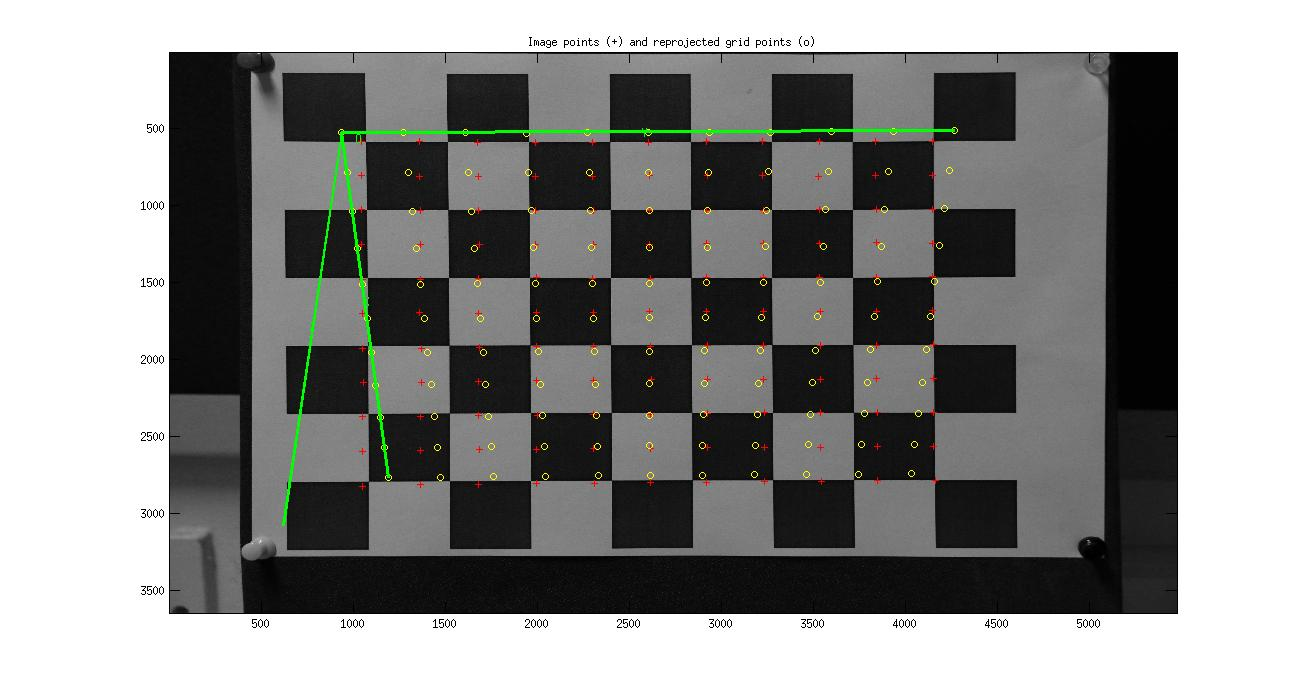
\includegraphics[width=1\textwidth]{wireFrame5456.jpg}\hfill
\end{figure}

\begin{figure}[htp]
\centering
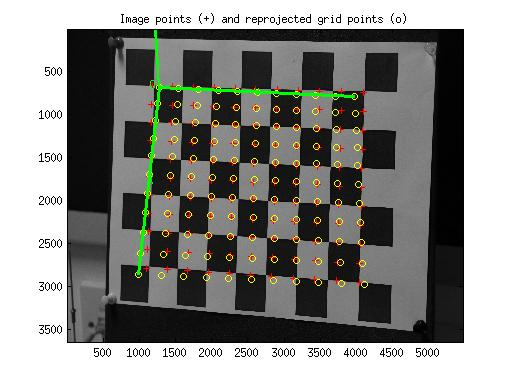
\includegraphics[width=1\textwidth]{wireFrame5457.jpg}\hfill
\end{figure}

\begin{figure}[htp]
\centering
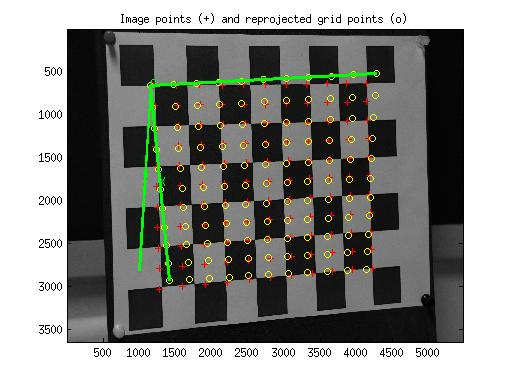
\includegraphics[width=1\textwidth]{wireFrame5458_2.jpg}\hfill
\end{figure}

\clearpage


\section{Personal Camera Calibration}
\subsection{DLT}
\subsection{Code}
\begin{lstlisting}
 close all;
 I = imread('Checkerboard4.jpg');
 figure;
 imshow(I);
 I = rgb2gray(I);
 C = corner(I, 'harris');
 figure;
 imshow(I);
 hold on;
 plot(C(100:104,1),C(100:104,2),'r*');
 plot(C(105,1), C(105,2), 'r*');

 imgCoord = [C(100:104,:), ; C(106,:)];
 imgCoord = [imgCoord, repmat(1,6,1)]
 worldCoord = [15.7, 0.7,0,1;
               11.2, 6.3, 0,1;
               1.0, 6.3, 3.4, 1;
               2.1, 6.3, 5.6, 1;
               18, 0.7, 0, 1;
               5.7, 6.3, 4.6,1];
           
           DLT(imgCoord, worldCoord)       

\end{lstlisting}

\subsection{Input}
To estimate the camera parameters, the following  image of a checkerboard is used
\begin{figure}[htp]
\centering
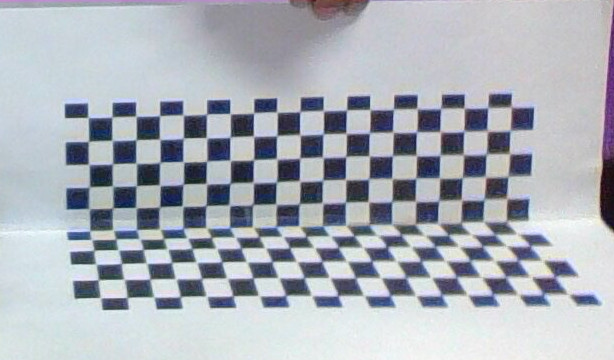
\includegraphics[width=1\textwidth]{Checkerboard4.jpg}\hfill
\end{figure}
\clearpage

After corner points are detected by Harris corner detector, the camera parameters are estimated.
\begin{figure}[htp]
\centering
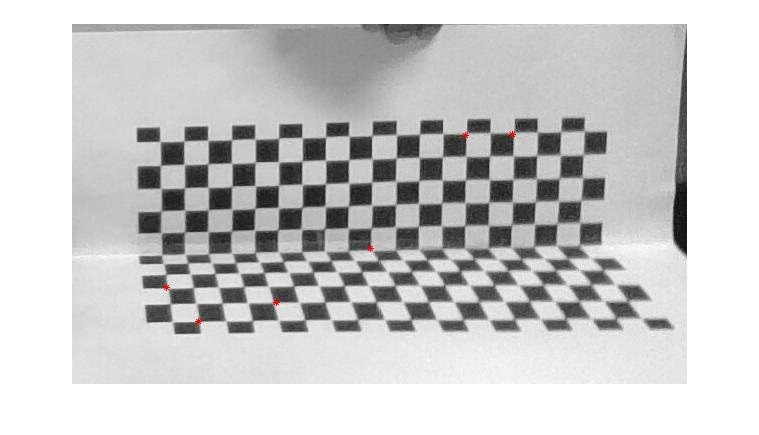
\includegraphics[width=1\textwidth]{harris.jpg}\hfill
\end{figure}
\clearpage
The world coordinates are as follows:
\begin{lstlisting} 
  15.7, 0.7,0,1;
  11.2, 6.3, 0,1;
  1.0, 6.3, 3.4,1;
  2.1, 6.3, 5.6, 1;
  18, 0.7, 0, 1;
  5.7, 6.3, 4.6,1
   \end{lstlisting}
   
\subsection{Output}
The actual image coordinates as calculated by Harris Corner Detector is 
\begin{lstlisting}
  393   112     1
  298   225     1
   95   264     1
  127   298     1
  440   111     1
  204   279     1
   \end{lstlisting}
   
The estimated image coordinates of after projection is
\begin{lstlisting} 
  393.9466  114.3111    1.0000
  297.6838  224.1224    1.0000
   95.2003  264.3033    1.0000
  125.8565  294.3272    1.0000
  439.0968  108.6573    1.0000
  205.2880  283.4391    1.0000
   \end{lstlisting}

\subsection{Projection Matrix P}
\begin{tabular}{|c|c|c|c|}
\hline
  -0.0410  &  0.0902  &  0.0032  & -0.7749 \\
    0.0150 & -0.0072  & -0.0007  & -0.6240 \\
    0.0001  &  0.0003  &  0.0001 &  -0.0046 \\
    \hline
\end{tabular}

\subsubsection{Intrinsic Parameter K}
\begin{tabular}{|c|c|c|}
\hline
 -0.0237 &  -0.0611 &   0.0743 \\
         0   & 0.0163  &  -0.0037 \\
         0  &       0  &  0.0003\\
\hline
\end{tabular}

\subsubsection{Extrinsic Parameter R}
\begin{tabular}{|c|c|c|}
\hline
  -0.1225 & -0.3521 &   0.9279 \\
    0.9705 &  -0.2381  &  0.0377 \\
    0.2077 &   0.9052  &  0.3709\\
\hline
\end{tabular}

\subsubsection{Extrinsic Parameter C}
\begin{tabular}{|c|c|c|}
\hline
  -55.1245 &
  -36.4208 &
   77.3984 \\
 \hline
\end{tabular}

\subsection{RANSAC}
\subsection{Code}
\begin{lstlisting}
  close all;
 I = imread('Checkerboard4.jpg');
 figure;
 imshow(I);
 I = rgb2gray(I);
 C = corner(I, 'harris');
 figure;
 imshow(I);
 hold on;
 plot(C(100:104,1),C(100:104,2),'r*');
 plot(C(106:114,1), C(106:114,2),'r*');
 
 imgCoord = [C(100:104,:), ; C(106:114,:)];
 imgCoord = [imgCoord, repmat(1,size(imgCoord,1),1)]
 worldCoord = [15.7, 0.7,0,1;
              11.2, 6.3, 0,1;
              1.0, 6.3, 3.4, 1;
              2.1, 6.3, 5.6, 1;
              18, 0.7, 0, 1;
              5.7, 6.3, 4.6,1;
              13.6, 4.1, 1,1;
              3.4,5.2,0,1;
              7.8, 6.3, 1,1;
              12.4,1.7,0,1;
              3.4, 2.9,0,1;
              5.7, 6.3, 6.4,1;
              0,6.3,1.1,1;
              4.5, 6.3,3.4,1];
          [p, K, R, c, imgEstimated] = RANSAC(imgCoord, worldCoord);
      

\end{lstlisting}

\subsection{Input}
To estimate the camera parameters, the following  image of a checkerboard is used
\begin{figure}[htp]
\centering
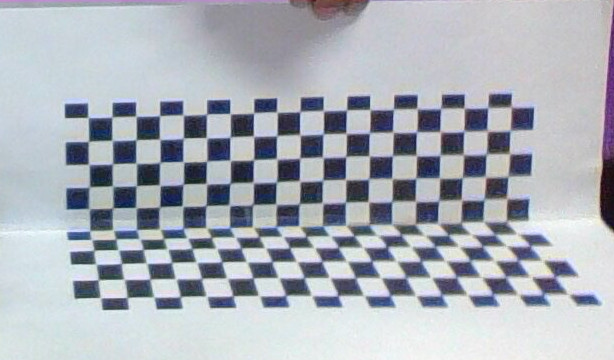
\includegraphics[width=1\textwidth]{Checkerboard4.jpg}\hfill
\end{figure}
\clearpage

After corner points are detected by Harris corner detector, the camera parameters are estimated.
\begin{figure}[htp]
\centering
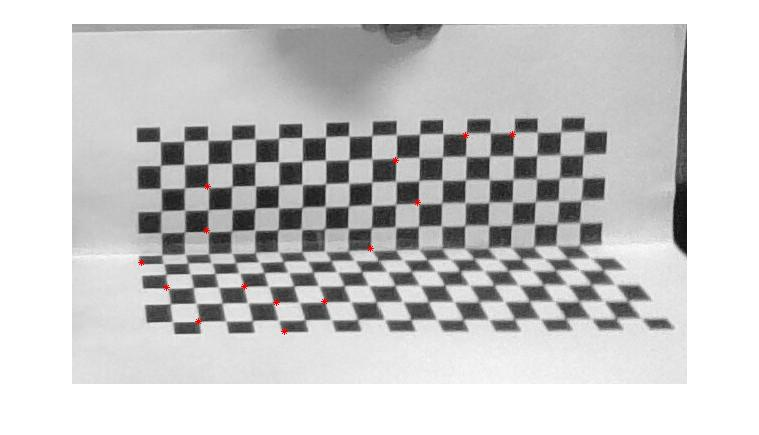
\includegraphics[width=1\textwidth]{harris2.jpg}\hfill
\end{figure}
\clearpage
The world coordinates are as follows:
\begin{lstlisting} 
  			  15.7, 0.7,0,1;
              11.2, 6.3, 0,1;
              1.0, 6.3, 3.4, 1;
              2.1, 6.3, 5.6, 1;
              18, 0.7, 0, 1;
              5.7, 6.3, 4.6,1;
              13.6, 4.1, 1,1;
              3.4,5.2,0,1;
              7.8, 6.3, 1,1;
              12.4,1.7,0,1;
              3.4, 2.9,0,1;
              5.7, 6.3, 6.4,1;
              0,6.3,1.1,1;
              4.5, 6.3,3.4,1
   \end{lstlisting}
   
\subsection{Output}
The RMS error of the estimated and actual image coordiantes, is  6.2812.

The actual image coordinates as calculated by Harris Corner Detector is 
\begin{lstlisting}
   393   112     1
   298   225     1
    95   264     1
   127   298     1
   440   111     1
   204   279     1
   345   179     1
   135   207     1
   252   278     1
   323   137     1
   136   163     1
   212   308     1
    70   239     1
   173   263     1

   \end{lstlisting}
   
The estimated image coordinates of after projection is
\begin{lstlisting} 
   389   113     1
   298   225     1
    95   264     1
   126   292     1
   440   111     1
   204   279     1
   357   190     1
   135   206     1
   231   237     1
   319   135     1
   136   163     1
   214   303     1
    70   239     1
   171   264     1
   \end{lstlisting}

\subsection{Projection Matrix P}
\begin{tabular}{|c|c|c|c|}
\hline
    0.1305  & -0.0095 &   0.0002  &  0.5308 \\
   -0.0104  &  0.1189 &   0.0313  &  0.8281 \\
   -0.0000  & -0.0001 &  -0.0002 &   0.0073 \\
    \hline
\end{tabular}

\subsubsection{Intrinsic Parameter K}
\begin{tabular}{|c|c|c|}
\hline
    -0.1222 &  0.0391   & 0.0258 \\
         0  & -0.1057  &  0.0637 \\
         0   &      0 &  -0.0002\\
\hline
\end{tabular}

\subsubsection{Extrinsic Parameter R}
\begin{tabular}{|c|c|c|}
\hline
   -0.9482 &  -0.1556 &   0.2771 \\
    0.2302 &  -0.9373  &  0.2615 \\
    0.2190 &  0.3118  &  0.9246\\
\hline
\end{tabular}

\subsubsection{Extrinsic Parameter C}
\begin{tabular}{|c|c|c|}
\hline
  5.7456  &
   21.6508 &
  -53.9559\\
 \hline
\end{tabular}

\subsection{Zhang Method}
OpenCv's implementation of Zhang's method is used for this experiment. A video of checkerboard print out is the input to the program. The results produce the laptop camera parameters.

\subsection{Input}
The input to opencv's Zhang method was a video captured by my laptop camera. The configuration file was modified with the following parameters:
\begin{lstlisting}[language=matlab]
<BoardSize_Width> 19</BoardSize_Width>
  <BoardSize_Height>11</BoardSize_Height>
  
  <!-- The size of a square in some user defined metric system (pixel, millimeter)-->
  <Square_Size>29</Square_Size>
  \end{lstlisting}
  
A screenshot for the input video is as follows:
\begin{figure}[htp]
\centering
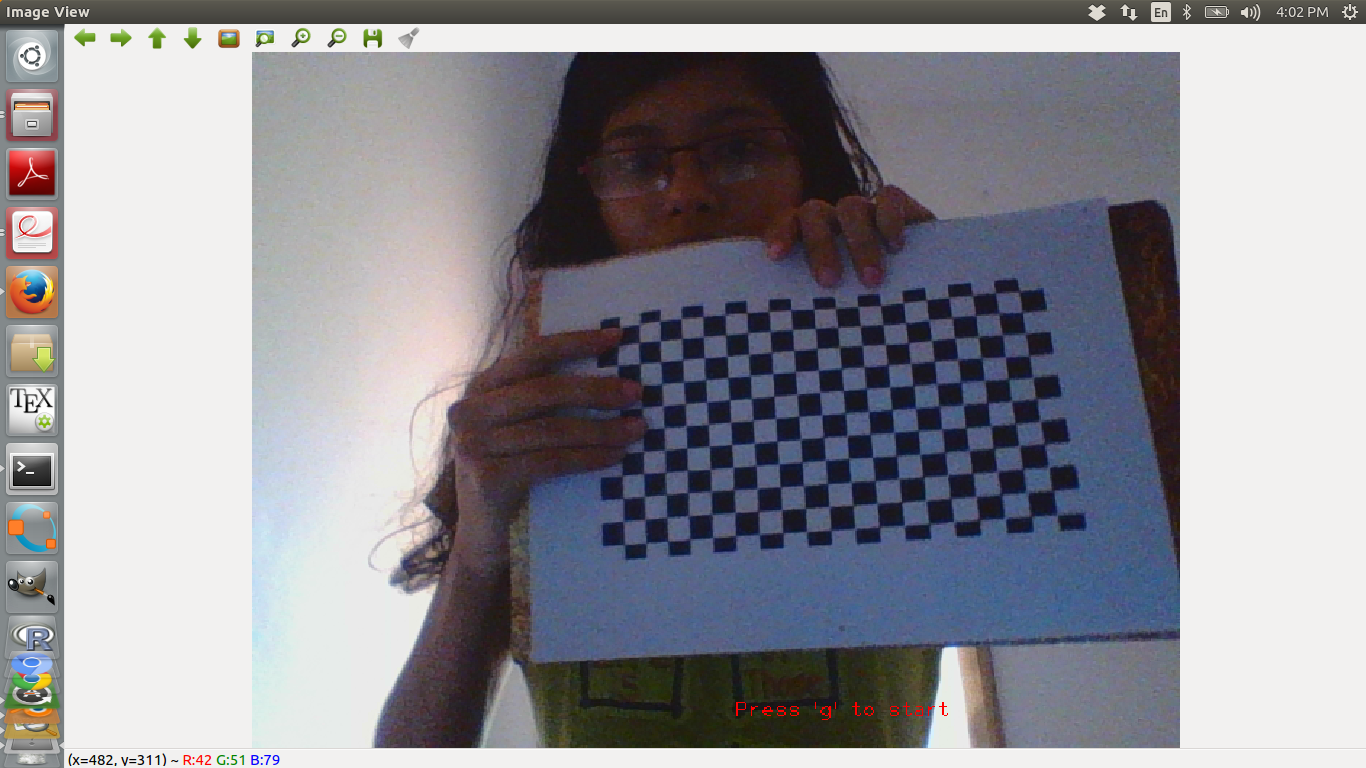
\includegraphics[width=1\textwidth]{inputZhang.png}\hfill
\end{figure}
\clearpage


\subsection{Output}
The output was produced in an xml file.

\subsection{Average Re-Projection Error}
The average re-projection error is 1.8200765999238961.
\subsection{Per view Re-projection Error}
\begin{tabular}{|c|c|c|c|c|}
\hline
view & 1 & 2 & 3 & 4 \\
Error & 2.55904078e+00 & 3.35413074e+00 & 1.39477491e+00 & 1.79452944e+00 \\
\hline \hline
view & 5 & 6 & 7 & 8 \\
Error & 2.17249346e+00 & 2.10425711e+00 & 1.28227234e+00 & 1.40593469e+00 \\
\hline \hline
view & 9 & 10 & 11 & 12 \\
Error &  1.28024423e+00 & 1.32076836e+00 & 1.32660282e+00 &  1.34940219e+00 \\
\hline \hline
view & 13 & 14 & 15 &  \\
 Error &  1.35390007e+00 & 1.54767573e+00 & 1.66267991e+00 &  \\
 \hline
\end{tabular}
 
    
   


\subsubsection{Intrinsic Parameter K}
\begin{tabular}{|c|c|c|}
\hline
610.5925  & 0 & 319.5 \\
0 &  610.59251 & 239.5 \\
0 & 0 & 1\\
\hline
\end{tabular}

\subsubsection{Extrinsic Parameters}
There are 15 rotation matrices for the 15 frames used to calibrate the camera.

\subsubsection{Rotation Matrix 1}
\begin{tabular}{|c|c|c|}
\hline
  
 0.9944153858813619 &  0.04644720256834592 &  0.09476654312571038 \\ 
  0.06183190592599129 &  0.984102379779916 &  0.1664912055367049 \\ 
  0.08552692986411618 &  0.1714210123791159 &  0.9814784667953432
\\ 
\hline
\end{tabular}
\subsubsection{Rotation Matrix 2}
\begin{tabular}{|c|c|c|}
\hline

  
 0.9877072850168229 &  0.02189517931141388 &  0.1547737711875546 \\ 
  0.04214306369463074 &  0.9907773096138155 &  0.1287799865539668 \\ 
  0.150526679718669 &  0.1337195717811369 &  0.9795206964712602
\\ 
\hline
\end{tabular}
\subsubsection{Rotation Matrix 3}
\begin{tabular}{|c|c|c|}
\hline

  
 0.9785785947648702 &  0.01139635247293982 &  0.2055579164574416 \\ 
  0.02368345942061683 &  0.9856061664806332 &  0.1673904965797713 \\ 
  0.2045067911290087 &  0.1686730794930328 &  0.9642231923348727
\\ 
\hline
\end{tabular}
\subsubsection{Rotation Matrix 4}
\begin{tabular}{|c|c|c|}
\hline

  
 0.9889353151907873 &  0.03763356515977519 &  0.1434944498643178 \\ 
  0.01654880806631006 &  0.9892358932535118 &  0.1453907990572682 \\ 
  0.1474214343984032 &  0.1414074335821547 &  0.9789131005393819
\\ 
\hline
\end{tabular}
\subsubsection{Rotation Matrix 5}
\begin{tabular}{|c|c|c|}
\hline

  
 0.9932638515409313 &  0.03054604568229187 &  0.1117759379976311 \\ 
  0.01435745801753814 &  0.9896381475906408 &  0.1428642720649206 \\ 
  0.1149816708060444 &  0.1402970987816226 &  0.9834103616761981
\\ 
\hline
\end{tabular}
\subsubsection{Rotation Matrix 6}
\begin{tabular}{|c|c|c|}
\hline

  
 0.9889313685214007 &  0.04631375490558493 &  0.1409602229741957 \\ 
  0.02677026419461661 &  0.9901388915865775 &  0.1375075573292396 \\ 
  0.1459386902412791 &  0.1322119944416886 &  0.9804192405376442
\\ 
\hline
\end{tabular}
\subsubsection{Rotation Matrix 7}
\begin{tabular}{|c|c|c|}
\hline

  
 0.9860060464987002 &  0.0514562035824 &  0.1585696546659849 \\ 
  0.02715618304314679 &  0.9880439617364435 &  0.151761890468854 \\ 
  0.1644828805393747 &  0.1453319950631654 &  0.9756146745618527
\\ 
\hline
\end{tabular}
\subsubsection{Rotation Matrix 8}
\begin{tabular}{|c|c|c|}
\hline

  
 0.9884177304001679 &  0.04903547399095185 &  0.1436172431188668 \\ 
  0.02453856250354929 &  0.9855470760410654 &  0.1676150943595648 \\ 
  0.1497606396248374 &  0.1621495704508313 &  0.9753354641464497
\\ 
\hline
\end{tabular}
\subsubsection{Rotation Matrix 9}
\begin{tabular}{|c|c|c|}
\hline

  
 0.9858948001064214 &  0.04865544162448861 &  0.1601377254848005 \\ 
  0.0254425131766876 &  0.98926018164094 &  0.1439339138041776 \\ 
  0.165421043541544 &  0.1378293909877728 &  0.9765443857467853
\\ 
\hline
\end{tabular}
\subsubsection{Rotation Matrix 10}
\begin{tabular}{|c|c|c|}
\hline

  
 0.9864359650763496 &  0.04919714638842972 &  0.1566005350920815 \\ 
  0.02520419825167085 &  0.9881114263639688 &  0.1516593468252245 \\ 
  0.1621999851861316 &  0.1456552432156106 &  0.9759486230993003
\\ 
\hline
\end{tabular}
\subsubsection{Rotation Matrix 11}
\begin{tabular}{|c|c|c|}
\hline

  
 0.9905671015421 &  0.04655920125705018 &  0.128876134799226 \\ 
  0.02617475386368812 &  0.9874790952590239 &  0.1555632305096387 \\ 
  0.1345053887495148 &  0.1507225172451851 &  0.9793829808571398
\\ 
\hline
\end{tabular}
\subsubsection{Rotation Matrix 12}
\begin{tabular}{|c|c|c|}
\hline

  
 0.9861447970862782 &  0.0515363816618411 &  0.157678281779287 \\ 
  0.02753010035394438 &  0.9881802201124655 &  0.1508043306837737 \\ 
  0.1635864687379887 &  0.1443740071608607 &  0.9759075844065107
\\ 
\hline
\end{tabular}
\subsubsection{Rotation Matrix 13}
\begin{tabular}{|c|c|c|}
\hline

  
 0.9850143337507793 &  0.05407819465414048 &  0.1637751848371947 \\ 
  0.0290230116137913 &  0.9880035153001969 &  0.1516796576714206 \\ 
  0.1700130203907164 &  0.14465338785318 &  0.9747671364383512
\\ 
\hline
\end{tabular}
\subsubsection{Rotation Matrix 14}
\begin{tabular}{|c|c|c|}
\hline

  
 0.9870972564948877 &  0.05471295201660221 &  0.150484215457619 \\ 
  0.03136552065742539 &  0.9876730612924687 &  0.1533562131478606 \\ 
  0.1570197768886287 &  0.146657481496146 &  0.9766454693424083
\\ 
\hline
\end{tabular}
\subsubsection{Rotation Matrix 15}
\begin{tabular}{|c|c|c|}
\hline

  
 0.9888288940751532 &  0.05372955742912307 &  0.1390343587052494 \\ 
  0.03184827615672366 &  0.9873905459629507 &  0.1550664278586154 \\ 
  0.1456128618905434 &  0.1489061597163014 &  0.9780714953675875
\\ 
\hline
\end{tabular}

\subsection{Output Image}
The screenshot of the calibration video is as follows
\begin{figure}[htp]
\centering
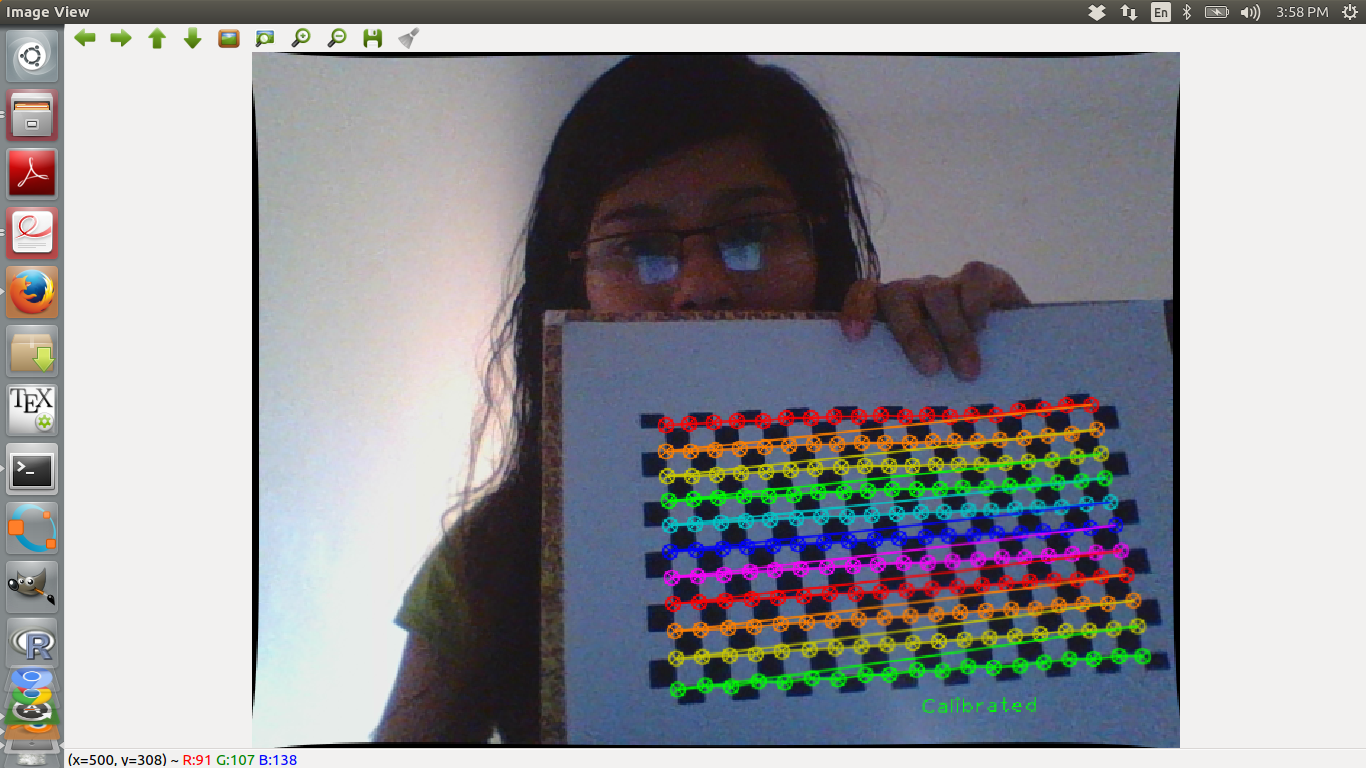
\includegraphics[width=1\textwidth]{outputZhang.png}\hfill
\end{figure}
\clearpage

\end{document}
